\documentclass[10pt,a4paper]{article}
\usepackage[utf8]{inputenc}
\usepackage{amsmath}
\usepackage{amsfonts}
\usepackage{amssymb}
\usepackage{ulem}
\usepackage{graphicx}
\author{GIMENEZ Florian}
\title{Compte Rendu TP1 Modélisation Identification et Commande}

\begin{document}
\normalem

\section{Traveaux Pratique 1}

\subsection{Programme affichant "Bonjour"}
\subsubsection{Code}
	\begin{figure}[h]
	\begin{center}
	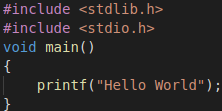
\includegraphics[scale=.4]{images/bonjour_c}
	\end{center}
	\caption{Programme C pour le programme Hello World}
	\end{figure}
\paragraph{}
    Pour afficher "Hello World" nous devons simplement placer un \emph{printf}.

\subsubsection{Résultat}
	\begin{figure}[h]
	\begin{center}
	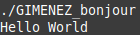
\includegraphics[scale=.4]{images/bonjour_ex}
	\end{center}
	\caption{Résultat du Programme \emph{bonjour}}
	\end{figure}

\subsection{Calcul Aire d'un disque}
\subsubsection{Code}
    \begin{figure}[h]
	\begin{center}
	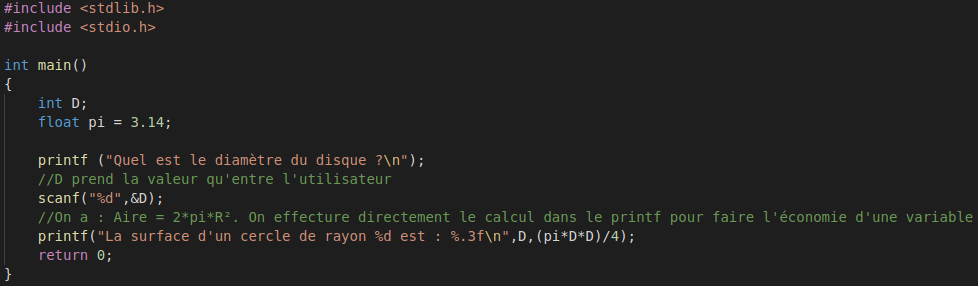
\includegraphics[scale=.3]{images/disque_c}
	\end{center}
	\caption{Programme C pour le calcul de l'aire d'un Disque}
	\end{figure}
\paragraph{}
Ici nous avons demandé le diamètre d'un disque pour pouvoir calculer son aire. Nous avons aussi affiché le résultat avec 3 
chiffres après la virgule. Nous avons aussi fait le calcul directement dans le \emph{printf}, pour faire l'économie d'une 
variable et rendre le programme plus lisible.
\subsubsection{Résultat}
	\begin{figure}[h]
	\begin{center}
	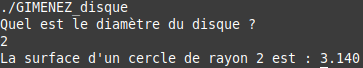
\includegraphics[scale=.3]{images/disque_ex}
	\end{center}
	\caption{Résultat du Programme \emph{disque}}
	\end{figure}


\subsection{Signe du produit}
\subsubsection{Code}
    \begin{figure}[h]
	\begin{center}
	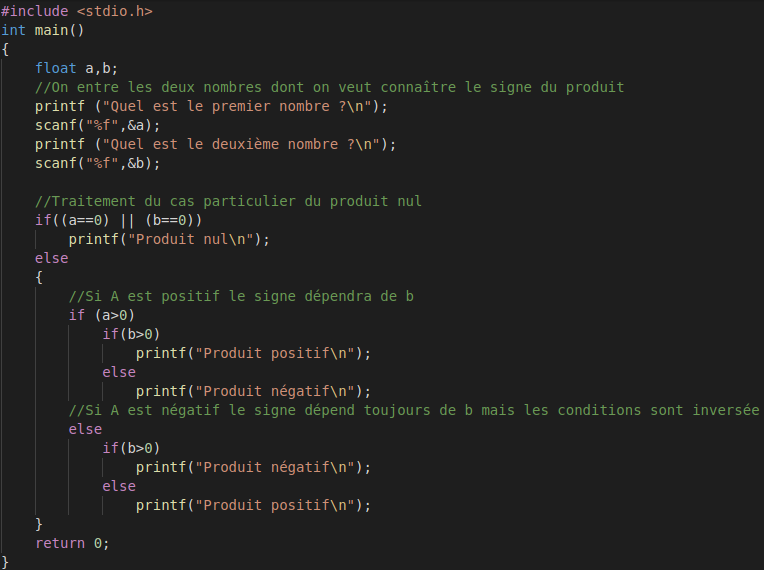
\includegraphics[scale=.3]{images/produit_c}
	\end{center}
	\caption{Programme C pour la déterminaion du signe d'un produit}
	\end{figure}
\paragraph{}
	Nous cherchons à determiner si le signe résultant du produit de deux nombres sera positif
	ou négatif. Pour cela nous testons tout d'abord le cas particulier où l'un des deux 
	nombre est nul. Par la suite en fonction du signe des nombres on pourra déterminer le signe 
	du résultat.
\subsubsection{Résultat}
	\begin{figure}[h]
	\begin{center}
	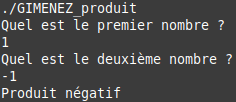
\includegraphics[scale=.3]{images/produit_ex}
	\end{center}
	\caption{Résultat du Programme \emph{produit}}
	\end{figure}


\subsection{Polynôme}
\subsubsection{Code}
	\begin{figure}[h]
	\begin{center}
	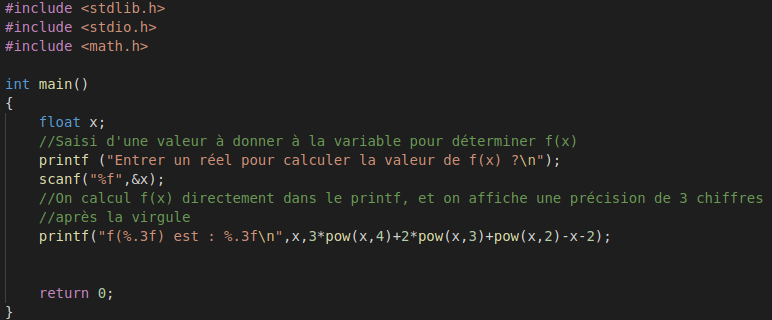
\includegraphics[scale=.3]{images/polynome_c}
	\end{center}
	\caption{Programme C pour le calcul d'une fonction}
	\end{figure}
\paragraph{}
	Nous souhaitons créer un programme permettant de calculer la valeur de la fonction 
	\emph{f} pour un \emph{x} donné. Nous avons utilisé la fonction \emph{power} de la librairie 
	math.h, pour effectuer les calculs de puissance.   
\subsubsection{Résultat}
	\begin{figure}[h]
	\begin{center}
	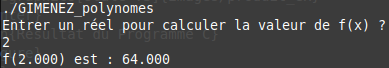
\includegraphics[scale=.3]{images/polynome_ex}
	\end{center}
	\caption{Résultat du Programme \emph{polynome}}
	\end{figure}


\subsection{Conversion de secondes vers le format HH:MM:SS}
\subsubsection{Code}
	\begin{figure}[h]
	\begin{center}
	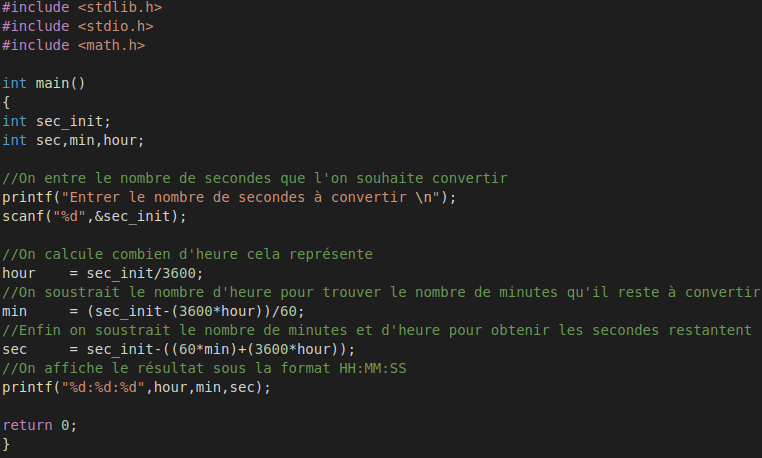
\includegraphics[scale=.3]{images/conversion_c}
	\end{center}
	\caption{Programme C pour la conversion d'un nombre de secondes en nombres d'heures, minutes et secondes}
	\end{figure}
\paragraph{}
	Nous avons ici créer un programme qui prend en entrées un nombre de secondes et qui l'a converti 
	en nombres d'heures, de minutes, et de secondes. On notera que pour ce programme toute les 
	divsions sont des divisions entière où on laisse le soin au compilateur d'arrondir les valeurs.
\subsubsection{Résultat}
	\begin{figure}[h]
	\begin{center}
	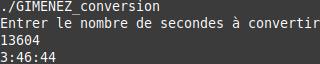
\includegraphics[scale=.3]{images/conversion_ex}
	\end{center}
	\caption{Résultat du Programme \emph{conversion}}
	\end{figure}

\subsection{Calculatrice}
\subsubsection{Code}
	\begin{figure}[h]
	\begin{center}
	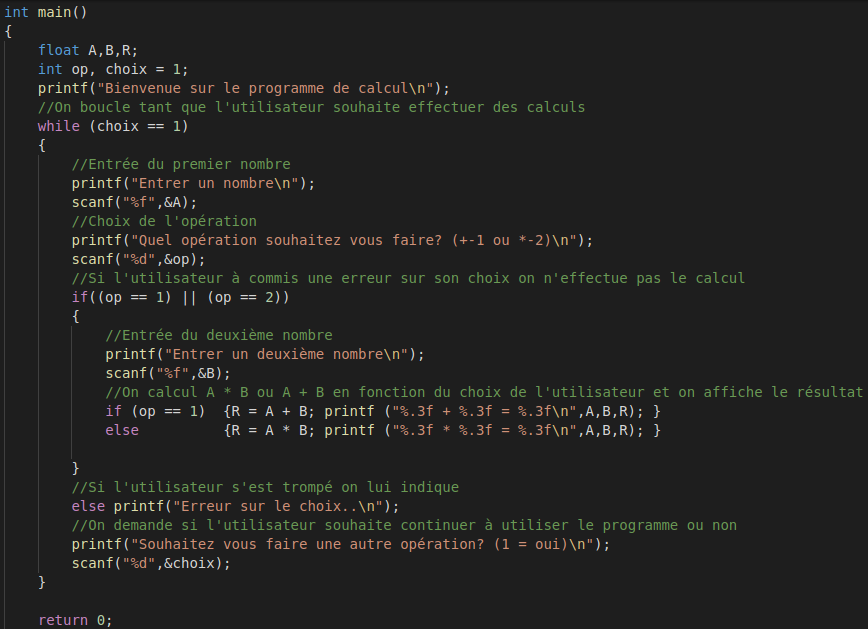
\includegraphics[scale=.3]{images/calculatrice_c}
	\end{center}
	\caption{Programme C pour la création d'une calculatrice}
	\end{figure}
\paragraph{}
	Ici nous avons créé un programme qui nous permet d'entrer deux nombres et d'effectuer une opération mathématique (+ ou *). 
	Nous demandons alors à l'utilisateur d'entrer un premier nombre puis un opération et enfin un deuxième nombre. On vérifie que 
	l'utilisateur à bien un opération valable.
\subsubsection{Résultat}
	\begin{figure}[h]
	\begin{center}
	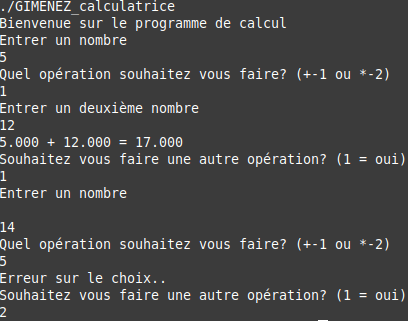
\includegraphics[scale=.3]{images/calculatrice_ex}
	\end{center}
	\caption{Résultat du Programme \emph{calculatrice}}
	\end{figure}

\section{Traveaux Pratique 2}

\subsection{Factorielle}
\subsubsection{Code}
	\begin{figure}[h]
	\begin{center}
	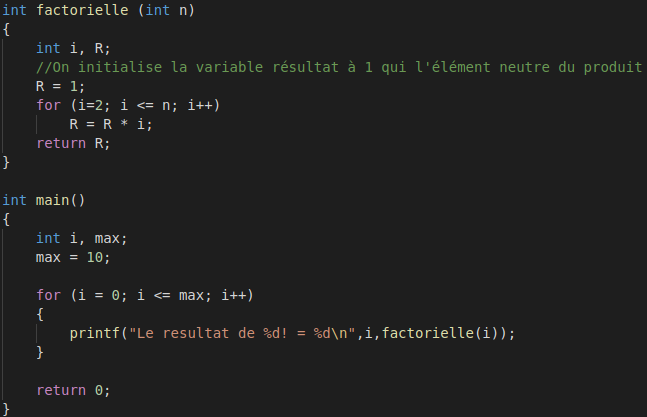
\includegraphics[scale=.3]{images/factorielle_c}
	\end{center}
	\caption{Programme C du calcul de la facotrielle}
	\end{figure}
\paragraph{}
	Le but de ce code était de pouvoir calculer la factorielle d'un nombre et aussi d'afficher les résultats intermédiaires. 
	On a ici créer une fonction pour faciliter la construction du texte. On a donc plus qu'a récupérer les valeurs et les afficher.
	La construction de la fonction fait que pour 0!, on obtient bien 1 comme résultat.
\subsubsection{Résultat}
	\begin{figure}[h]
	\begin{center}
	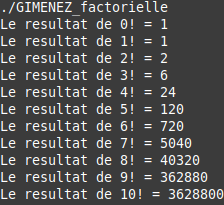
\includegraphics[scale=.3]{images/factorielle_ex}
	\end{center}
	\caption{Résultat du Programme \emph{factorielle}}
	\end{figure}

\end{document}